%%
%% This is file `sample-sigconf.tex',
%% generated with the docstrip utility.
%%
%% The original source files were:
%%
%% samples.dtx  (with options: `sigconf')
%%
%% IMPORTANT NOTICE:
%%
%% For the copyright see the source file.
%%
%% Any modified versions of this file must be renamed
%% with new filenames distinct from sample-sigconf.tex.
%%
%% For distribution of the original source see the terms
%% for copying and modification in the file samples.dtx.
%%
%% This generated file may be distributed as long as the
%% original source files, as listed above, are part of the
%% same distribution. (The sources need not necessarily be
%% in the same archive or directory.)
%%
%% The first command in your LaTeX source must be the \documentclass command.
\documentclass[sigconf]{acmart}
\usepackage{microtype}
\usepackage[utf8]{inputenc}
\usepackage{xcolor}
\usepackage{graphicx}
\usepackage{setspace}
\usepackage{enumerate}
\usepackage{multirow}
\usepackage{booktabs}
\usepackage{mathtools} 
\usepackage{subcaption}
\usepackage{caption}
\usepackage{tikz}
\usepackage{mdframed}
\usepackage{wrapfig}
\usepackage{caption}

\usepackage{oPlotSymbl}
%\usepackage{tikz}
%\newcommand*\circled[1]{\tikz[baseline=(char.base)]{
%		\node[shape=circle,draw,inner sep=2pt] (char) {#1};}}


% Remove indention for paragraphs?
\setlength{\parindent}{0pt}
% Microtype ist einfach super, aber lesen Sie
% unbedingt die Anleitung um das Folgende zu
% verstehen.

%\definecolor{cadmiumgreen}{rgb}{0.0, 0.42, 0.24}
%\definecolor{bostonred}{rgb}{0.8, 0.0, 0.0}

\definecolor{indigo}{rgb}{0.0, 0.25, 0.72}
\definecolor{indigo2}{rgb}{0.0, 0.25, 0.42}
\newcommand{\greybox}[1]{
	\begin{mdframed}[backgroundcolor=black!10!white,linewidth=0pt,backgroundcolor=indigo2!10,linewidth=0pt,innerleftmargin=5pt,innertopmargin=5pt]
		%\noindent
		#1
	\end{mdframed}
}

%% \BibTeX command to typeset BibTeX logo in the docs
%\AtBeginDocument{%
%  \providecommand\BibTeX{{%
%    \normalfont B\kern-0.5em{\scshape i\kern-0.25em b}\kern-0.8em\TeX}}}

%% Rights management information.  This information is sent to you
%% when you complete the rights form.  These commands have SAMPLE
%% values in them; it is your responsibility as an author to replace
%% the commands and values with those provided to you when you
%% complete the rights form.
%s\setcopyright{acmcopyright}
%\copyrightyear{2018}
%\acmYear{2018}
%\acmDOI{10.1145/1122445.1122456}

%% These commands are for a PROCEEDINGS abstract or paper.

% ACM Joint European Software Engineering Conference and Symposium on the Foundations of Software Engineering (ESEC/FSE)
\acmConference[ASE '20]{ASE '20: IEEE/ACM International Conference on Automated Software Engineering}{September 21--25, 2020}{Melbourne, Australia}
\acmBooktitle{ASE '20: IEEE/ACM International Conference on Automated Software Engineering, September 21--25, 2020, Melbourne, Australia}
%\acmPrice{15.00}
%\acmISBN{978-1-4503-XXXX-X/18/06}


%%
%% Submission ID.
%% Use this when submitting an article to a sponsored event. You'll
%% receive a unique submission ID from the organizers
%% of the event, and this ID should be used as the parameter to this command.
%%\acmSubmissionID{123-A56-BU3}

%%
%% The majority of ACM publications use numbered citations and
%% references.  The command \citestyle{authoryear} switches to the
%% "author year" style.
%%
%% If you are preparing content for an event
%% sponsored by ACM SIGGRAPH, you must use the "author year" style of
%% citations and references.
%% Uncommenting
%% the next command will enable that style.
%%\citestyle{acmauthoryear}

%%
%% end of the preamble, start of the body of the document source.
\begin{document}
	
	%\settopmatter{printacmref=false} 
	%\renewcommand\footnotetextcopyrightpermission[1]{}
	%%
	%% The "title" command has an optional parameter,
	%% allowing the author to define a "short title" to be used in page headers.
	\title[Identifying Software Performance Changes Across Variants and Versions]{\texorpdfstring{Identifying Software Performance Changes Across\\ Variants and Versions}{Identifying Software Performance Changes Across Variants and Versions}}
	
	%%
	%% The "author" command and its associated commands are used to define
	%% the authors and their affiliations.
	%% Of note is the shared affiliation of the first two authors, and the
	%% "authornote" and "authornotemark" commands
	%% used to denote shared contribution to the research.
	
	\author{Stefan Mühlbauer}
	\affiliation{%
		\institution{Leipzig University,}
		%\city{Doimukh}
		\country{Germany}}
	
	\author{Sven Apel}
	\affiliation{%
		\institution{Saarland University,}
		%\city{Doimukh}
		\country{Germany}}
	
	\author{Norbert Siegmund}
	\affiliation{%
		\institution{Leipzig University,}
		%\city{Doimukh}
		\country{Germany}}
	%%
	%%
	%% By default, the full list of authors will be used in the page
	%% headers. Often, this list is too long, and will overlap
	%% other information printed in the page headers. This command allows
	%% the author to define a more concise list
	%% of authors' names for this purpose.
	%\renewcommand{\shortauthors}{Trovato and Tobin, et al.}
	
	\copyrightyear{2020}
	\acmYear{2020}
	\setcopyright{acmcopyright}\acmConference[ASE '20]{35th IEEE/ACM International Conference on Automated Software Engineering}{September 21--25, 2020}{Virtual Event, Australia}
	\acmBooktitle{35th IEEE/ACM International Conference on Automated Software Engineering (ASE '20), September 21--25, 2020, Virtual Event, Australia}
	\acmPrice{15.00}
	\acmDOI{10.1145/3324884.3416573}
	\acmISBN{978-1-4503-6768-4/20/09}
	
	\begin{CCSXML}
		<ccs2012>
		<concept>
		<concept_id>10011007.10010940.10011003.10011002</concept_id>
		<concept_desc>Software and its engineering~Software performance</concept_desc>
		<concept_significance>500</concept_significance>
		</concept>
		<concept>
		<concept_id>10010147.10010257.10010282.10011304</concept_id>
		<concept_desc>Computing methodologies~Active learning settings</concept_desc>
		<concept_significance>500</concept_significance>
		</concept>
		<concept>
		<concept_id>10011007.10011074.10011111.10011113</concept_id>
		<concept_desc>Software and its engineering~Software evolution</concept_desc>
		<concept_significance>500</concept_significance>
		</concept>
		</ccs2012>
	\end{CCSXML}
	
	\ccsdesc[500]{Software and its engineering~Software performance}
	\ccsdesc[500]{Computing methodologies~Active learning settings}
	\ccsdesc[500]{Software and its engineering~Software evolution}
	
	
	%%
	%% The abstract is a short summary of the work to be presented in the
	%% article.
	\begin{abstract}
		We address the problem of identifying performance changes in the evolution of configurable software systems. Finding optimal configurations and configuration options that influence performance is already difficult, but in the light of software evolution, configuration-dependent performance changes may lurk in a potentially large number of different versions of the system.
		
		In this work, we combine two perspectives---variability and time---into a novel perspective. We propose an approach to identify con\-figuration-dependent performance changes retrospectively across the software variants and versions of a software system. In a nutshell, we iteratively sample pairs of configurations and versions and measure the respective performance, which we use to update a model of likelihoods for performance changes. Pursuing a search strategy with the goal of measuring selectively and incrementally further pairs, we increase the accuracy of identified change points related to configuration options and interactions.
		
		We have conducted a number of experiments both on controlled synthetic datasets as well as in real-world scenarios with different software systems. Our evaluation demonstrates that we can pinpoint performance shifts to individual configuration options and interactions as well as commits introducing change points with high accuracy and at scale. Experiments on three real-world systems explore the effectiveness and practicality of our approach.
		
	\end{abstract}
	
	%%
	%% The code below is generated by the tool at http://dl.acm.org/ccs.cfm.
	%% Please copy and paste the code instead of the example below.h
	%%
	%% Keywords. The author(s) should pick words that accurately describe
	%% the work being presented. Separate the keywords with commas.
	\keywords{software performance, software evolution, configurable software systems, machine learning, active learning}
	
	%% A "teaser" image appears between the author and affiliation
	%% information and the body of the document, and typically spans the
	%% page.
	
	
	%%
	%% This command processes the author and affiliation and title
	%% information and builds the first part of the formatted document.
	\maketitle
	
	
	\section{Introduction}
	%\paragraph{\bfseries What is the problem?}
	Software performance plays a crucial role in users' perception of software quality.
	Excessive execution times, low throughput, or otherwise unexpected performance without added value can render software systems unusable.
	Poor performance is often a symptom of deficiencies in particular software components or the overall software architecture.
	Changes in the observed performance of a software system can be attributed to changes to the software at different levels of granularity (architecture, code, etc.).
	
	% Das problem sind performance bugs in confi systems
	Typically, modern software systems provide configuration options to enable users and admins  customizing behavior to meet different user requirements.
	Configuration options usually correspond to pieces of selectable functionality (features), which contribute to overall performance with different proportions.
	That is, different configurations of a software system exhibit different performance characteristics depending on configuration decisions made by the user.
	
	Performance changes during software evolution---intended or not---can affect all or only a subset of configurations since changes to a software system often relate to a particular configuration option or set of options.
	This is why performance bugs are rarely visible in default configurations, but revealed only in certain configurations~\cite{hanEmpiricalStudyPerformance2016}.
	If undetected, such perennial bugs can persist for the lifetime of a software system as software evolves.
	Adding this \emph{technical debt} constantly can accumulate and entail trends of degrading performance quality~\cite{guoGeneticAlgorithmOptimized2011}.
	
	Performance assessment and estimation is a resource-intense task with many possible pitfalls prevailing.
	Best practices for conducting performance measurements emphasize a dedicated and separated hardware setup to prevent measurement bias by side-processes and, subsequently, obtain reproducible results~\cite{molyneauxArtApplicationPerformance2015}.	% performance measurement
	What is often overlooked is the fact that most software systems are configurable, which introduces another layer of complexity.
	Due to combinatorics, even for a small number of configuration options, the range of possible valid configurations renders exhaustive measurements infeasible.
	%Most problems involving configuration options, such as finding a configuration with optimal performance~\cite{ohFindingNearoptimalConfigurations2017,nairFlash18} or estimating the influence on performance of an individual option~\cite{siegmundPredictingPerformanceAutomated2012,siegmundPerformanceinfluenceModelsHighly2015,sarkarCostEfficientSamplingPerformance,haDeepPerf2019}.
	
	%\paragraph{\bfseries Why has it not been solved before?}
	%Our goal is to identify changes in the performance histories of configurable software systems and pinpoint them to a specific option or interaction. For example, a patch of a certain feature is likely to affect only configurations where such feature is selected.
	%In essence, we face a huge combinatorial problem for performance-change detection: code changes across software versions and behavioral changes across software variants.
	
	Our goal is to enable the \emph{retrospective} detection of changes in the performance of configurable software systems and pinpoint them to a specific option or interaction. For example, a patch of a certain feature is likely to affect only configurations where such feature is selected. 
	We would like to know in which revision this patch was introduced and which features were affected.
	Many software systems are configurable, but have no performance regression testing routine set in place. 
	To uncover performance deficiencies that emerged from revisions in the past development history, it is infeasible to test each and every commit and configuration. 
	In essence, we face a combinatorial explosion along two dimensions: time (versions) and configuration space (variants).
	\emph{First}, we aim at finding changes in software performance from one version to another.
	The detection of such changes is referred to as \emph{change point detection}~\cite{daly_industry_2020,cityIdentifying2014,huang_performance_2014,muhlbauer_accurate_2019,sandoval_alcocer_learning_2016,alcocer_prioritizing_2020}.
	The main limiting factor is that exhaustive measurements across the configuration space are neither available nor feasible~\cite{white_selecting_2009}.
	Change point detection techniques with both exhaustive measurement~\cite{cityIdentifying2014,daly_industry_2020} as well as limited data availability~\cite{sandoval_alcocer_learning_2016,alcocer_prioritizing_2020,huang_performance_2014,muhlbauer_accurate_2019} have been successfully applied to identify performance changes.
	\emph{Second}, we aim at associating performance changes (from one version to another) with particular configuration options or interactions among them.
	There is substantial work  regarding a related problem, which is estimating the influence of individual options on performance~\cite{siegmundPredictingPerformanceAutomated2012,siegmundPerformanceinfluenceModelsHighly2015,sarkarCostEfficientSamplingPerformance,haDeepPerf2019} for a single version of the software system, ignoring the temporal dimension. Instead of estimating the influence of options and interactions on performance, we want to know: Which option or interaction is \emph{responsible} for a particular change point in the version history of a software system?
	
	Our main idea is as follows: We address the configuration complexity of this problem by selecting representative sample sets of configurations.
	Then, we uniformly sample a constant number of commits for each configuration and conduct respective performance measurements.
	Based on these measurements, we learn a prediction model.
	For each configuration, we estimate the likelihood of each commit being a change point (i.e., that performance of some configurations changes abruptly compared to the previous commit).
	Next, we leverage similarities in the performance histories of configurations that share common options.
	Since we sample the commits for each configuration independently, we obtain for each change point many estimations using measurements of different commits.
	Overall, this allows us to obtain more accurate estimations of performance-changing commits with tractable effort.
	Based on a mapping from configurations to predicted change point probabilities for each configuration and commit, we derive the options responsible for each particular change point, which we call \emph{configuration-dependent change points}. 	
	In summary, we offer the following contributions:
	\begin{itemize}
		\item A novel technique to effectively identify shifts in performance of configurable software systems. It is able to pinpoint causative commits and affected configuration options with high accuracy and tractable effort.
		\item A feasibility demonstration of our approach by implementing an adaptive learning strategy to obtain accurate estimations with acceptable measurement cost.
		\item An evaluation using both synthetic and real-world performance data from three configurable software systems. Synthetic data let us assess our model and approach conceptually and at scale, whereas we are able to assess practicality with real-world data.
		\item A companion Web site\footnote{\url{https://github.com/AI-4-SE/Changepoints-Across-Variants-And-Versions/} or an archived version at \url{https://archive.softwareheritage.org/browse/origin/https://github.com/AI-4-SE/Changepoints-Across-Variants-And-Versions/}} providing supplementary material including a reference implementation of our approach, performance measurement data, and additional visualizations.
	\end{itemize}
	
	\section{Configuration-Dependent Change Points}
	Performance as a property emerges from a variety of factors.
	Besides external factors, including hardware setup or execution environment~\cite{ousterhout_always_2018}, the configuration  of a software system can influence performance to a large extent~\cite{siegmundPredictingPerformanceAutomated2012}.
	Most modern software systems exhibit configuration options that correspond to selectable pieces of functionality.
	With configuration options, we turn features on and off creating a variant of the software system.
	Depending on the configuration, different system variants with different behavior and performance can be derived.
	
	\subsection{Performance-Influence Models}\label{sec:pimodels}
	Consider the following running example of a database management system (DBMS) with two selectable features: \textsc{Encryption} and \textsc{compression}.
	Either feature adds execution time to the overall performance, but, if both features are selected, the execution time is smaller than the sum of the individual features' contribution to performance: Less data is encrypted if it is compressed beforehand.
	An \textit{interaction} in this setting is the combined effect of features \textsc{Encryption} and \textsc{compression}.
	We can assign each feature and interaction an \textit{influence} that it contributes to the overall performance, if selected. In our example, the individual influences of the two features are positive (increasing execution time), whilst the interaction's influence is negative (decreasing execution time).
	
	The influence of features on performance can be described using a \emph{performance-influence model}~\cite{siegmundPerformanceinfluenceModelsHighly2015}.
	A performance-influence model is a linear prediction model of the form $\Pi:C\rightarrow \mathbb{R}$, whereby $C$ denotes a configuration vector (assignment of concrete values to configuration options) and the estimate is a system variant's real-valued performance:

	\begin{align} \label{eq:pimodel}
		\begin{split}
		\Pi(c) = \beta^T c =  \begin{bmatrix}
		\beta_1\\
		\vdots \\
		\beta_{2^{\vert F\vert}}
		\end{bmatrix}^T \cdot \begin{bmatrix}
		c_1\\
		\vdots \\
		c_{2^{\vert F\vert}}
		\end{bmatrix}
		\end{split}
		\begin{split}
		\beta_i \in \mathbb{R}^{2^{|F|}}\\
		c_i \in \lbrace 0,1\rbrace^{2^{|F|}}
		\end{split}
	\end{align}
	
	$F$ denotes the set of all features. Our linear model has $\vert 2^F\vert$ terms, whereby each term $t \subseteq F$ corresponds to a subset of $F$ and is described by a coefficient $\beta_f$ and a configuration parameter $c_f$.
	Coefficients encode the performance-influence of features and interactions. $c$ is a vector and denotes the assignment of concrete values to configuration options or interactions. A configuration parameter $c_t$ evaluates to $1$, if all configuration options of the corresponding subset $t \subseteq F$ are selected, and $0$ otherwise. The empty set corresponds to the invariable core functionality of the software system. Singleton subsets correspond to individual features, compound subsets to interactions of features.
	
	For our DBMS example, we present a fully determined performance-influence model in Equation~\ref{eq:pimodel_dbms}. The first two terms correspond to the features \textsc{Encrpytion} and \textsc{Compression}, respectively. The third term respresents the interaction of both features. The configuration parameter $c_{\textsc{Compr}\land\textsc{Encrypt}}$ evaluates to $1$, if both $c_{\textsc{Encrypt}}$ and $c_{\textsc{Compr}}$ evaluate to $1$.
	That is, $c_{\textsc{Compr}\land\textsc{Encrypt}} \equiv c_{\textsc{Encrypt}} \cdot c_{\textsc{Compr}}$. In the last term, we omit the configuration parameter $c_\emptyset$, as this term represents invariable functionality.
	
	\begin{align} \label{eq:pimodel_dbms}
	\begin{split}
	\Pi_{\text{DBMS}}(c) =&~\beta_{\textsc{Encrpyt}} \cdot c_{\textsc{Encrpyt}} + \beta_{\textsc{Compr}} \cdot c_{\textsc{Compr}} \\
	+&~ \beta_{\textsc{Compr\ $\land$\ Encrpyt}} \cdot c_{\textsc{Compr\ $\land$\ Encrpyt}}
	+ \beta_{\emptyset}
	\end{split}
	\end{align}
	
	Prediction models of configuration-dependent performance of this form are not the only possible representation~\cite{guoVariabilityawarePerformancePrediction2013,haDeepPerf2019}, but linear models are easy to interpret~\cite{siegmundPerformanceinfluenceModelsHighly2015}.
	We review extensions and alternatives to linear performance-influence models in Section~\ref{sec:rw}.
	
	\subsection{Evolution of Performance Influences}
	Performance-influence models describe how features contribute to performance, but they do not allow for understanding configuration-dependent performance changes over time.
	We expand our DBMS example with a temporal dimension, considering a development history of hundred commits.
	In particular, we assume the following three events. (1) At commit 25, feature \textsc{Compression} has been modified, increasing the execution time; feature \textsc{Encryption} is introduced at commit 25 and can be combined with \textsc{Compression}. (2) At commit 50, the interaction of \textsc{Compression} and \textsc{Encryption} changes, resulting in an increased execution time. (3) At commit 80, the core functionality of the DBMS is refactored, which decreased execution time for all variants.
	\begin{figure}[ht!]
		%		\begin{subfigure}{\linewidth}
		\centering
		% include first image
		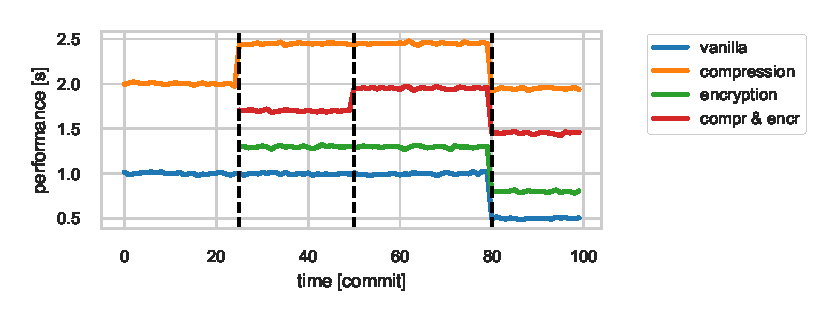
\includegraphics[width=\linewidth]{images/dbms_performance.eps}
		\caption{Performance of 4 variants with 3 change points}
		\label{fig:dbms_performance}
	\end{figure}
	
	The performance histories of the four valid variants in Figure~\ref{fig:dbms_performance} exhibit three change points: commits 25, 50, and 80. These change points, however, do not affect all configurations.
	For  instance, execution time decreases for all configurations at commit 80, but increases at commit 50 only for one configuration.
	Given this example, the target outcomes of our approach are (1) the locations of the three change points (commits 25, 50, and 80),  (2) the association of such commits to the features and interactions (\textsc{Compr}, $\text{\textsc{Compr}}\ \land\ \text{\textsc{Encrypt}}$), and the invariable functionality, respectively.
	
	\begin{figure}
		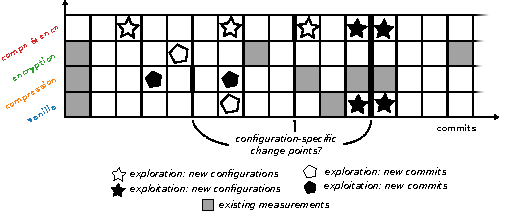
\includegraphics[width=0.5\textwidth]{images/sampling_plan}
		
		\caption{Active sampling strategies for a DBMS with 4 configurations}
		\label{fig:sampling plan}
	\end{figure}
	
	\subsection{Taming Complexity}
	A naive approach for identifying change points in the evolution of configurable software systems is to simply combine existing work on performance modeling of commit histories and performance prediction of software configurations.
	
	For our example, we could measure all variants for each commit building a performance-influence model per commit.
	Having 4 configurations and 100 commits, this would result in 400 measurements.
	Since the number of configurations grows exponentially with the number of features, we end up with $2^n$ times $T$ measurements where $n$ is the number of features and $T$ is the number of commits.
	Clearly, this does not scale along both dimensions: Already a few features would render even small commit histories intractable, and even small configuration spaces make this approach infeasible given realistic commit histories of a few thousands of commits.
	
	To obtain accurate estimations with a limited budget of measurements, we require a different approach. We propose an iterative and adaptive sampling approach. That is, we use an initial, but small sample set to explore the problem space and then increase the level of granularity at promising regions and dimensions (development history segments as well as individual features and interactions, in our case). 
	
	Based on the introductory DBMS example (cf. Figure~\ref{fig:dbms_performance}), we illustrate our sampling strategy in Figure~\ref{fig:sampling plan}. Here, each box depicts a possible measurement (i.e., a pair of a configuration and a commit). Black bars represent change points hidden in the software system‘s performance histories (i.e., measurements immediately before and after a change point are dissimilar). The current state of the sample set comprises all measurements that are filled in grey. 
	
	To include new measurements into the sample set, we consider the following situations. On the one hand, our sample set might already hint to some possible change points and associated configuration options. On the other hand, our sample set might be too sparse, such that we cannot infer some change points yet. To address this trade-off, we devise two strategies, exploration and exploitation, both of which address both configurations and commits. 
	
	 For \emph{exploitation}, we sample new measurements to verify guesses based on the current state. That is, in Figure~\ref{fig:sampling plan}, we might include the measurements depicted by black-filled symbols~($\starletfill$/$\pentagofill$). Black-filled stars~($\starletfill$) represent measurements that are of interest because we have already identified one change point for configuration \textsc{Compression}. We exploit this knowledge to test further configuration options involved in this change point. The black-filled pentagons~($\pentagofill$) represent measurements that are interesting, because we have identified another early change point for \textsc{Compression}, but within a rather broad range of commits. Thus, we include further measurements from that range to narrow down the possible range for this particular change point. 
	 
	 For \emph{exploration}, we might include the measurements denoted by white symbols~($\starlet$/$\pentago$). White stars~($\starlet$) represent measurements that explore new configurations. In our example, the interaction between \textsc{Compression} and \textsc{Encryption} is the only configuration left to be measured. We include several commits of a particular new configuration to unveil possible performance variation that indicates possible change points. White pentagons ($\pentago$) represent measurements that are of interest because they  increase the overall measurement coverage. We include measurements from large intervals of not yet measured commits, since possible change points can be hidden there.
	 
	These four strategies (exploration and exploitation of configurations and commits) prioritize measurements to be included next into the sample set. Adaptive sampling techniques have been successfully applied to obtain both performance-influence models~\cite{siegmundPredictingPerformanceAutomated2012,sarkarCostEfficientSamplingPerformance} and performance histories~\cite{muhlbauer_accurate_2019} before. However, it is unclear whether fewer measurements are sufficient to assess the performance-influence of configuration options and interactions with respect to version changes. This is what we address in this work.
		
	\section{An algorithm for change point detection}\label{sec:cpmodel}
	We propose an algorithm to detect substantial shifts in the performance of software configurations and associate them to individual commits and options or interactions. We lay out our approach as an iterative search across the commit history and configuration space. 
	
	We provide an overview of our approach in Figure~\ref{fig:overview}. 
	It starts with a small initial sample set of measurements (i.e., performance observations of varying configurations and varying commits). 
	Based on this sample set, it calculates for each configuration the likelihood of each commit being a change point. 
	
	Subsequently, our algorithm estimates a \emph{candidate solution}, which is a set of pairs of a commit and a configuration option. 
	Each of such pairs describes the estimated involvement of a configuration option in the shift of performance. 
	Interactions are conceived as multiple tuples with identical commits. That is, if a commit occurs in multiple tuples, each with different configuration options, this indicates that the shift arises from an interaction among two or more options. 
	Henceforth, we will refer to such pairs as \emph{associations}.
	
	After obtaining one candidate solution per search iteration, we augment the sample set of measurements with regard to two objectives: exploration and exploitation. 
	\emph{Exploration} aims at including previously unseen commits and configurations to improve coverage of the search space. 
	\emph{Exploitation} aims at including measurements in the sample set that, based on the previous candidate solution, may increase confidence in associations or rule out false positives (i.e., commits falsely identified as change points or options falsely associated with a commit). 
	As for exploitation, we make an informed decision of which measurements are to be included, whereas exploration is agnostic of previous candidate solutions.
	
	As each iteration yields a candidate solution, we keep track of associations in a \emph{solution cache} and repeatedly update the confidence of associations. 
	The rationale is not to lose previously identified change points, but at the same time, allow for removing identified changes points that are likely false positives due to new measurements.
	Some associations, especially in the beginning, might be influenced by sampling bias and can be removed if successive iterations do not repeatedly revisit these associations. 
	The algorithm terminates if the solution cache does not change for a number of iterations or a maximum number of iterations/measurements has been reached.
	In what follo, we present the steps of our approach in detail. 
	
	\begin{figure}[ht]
		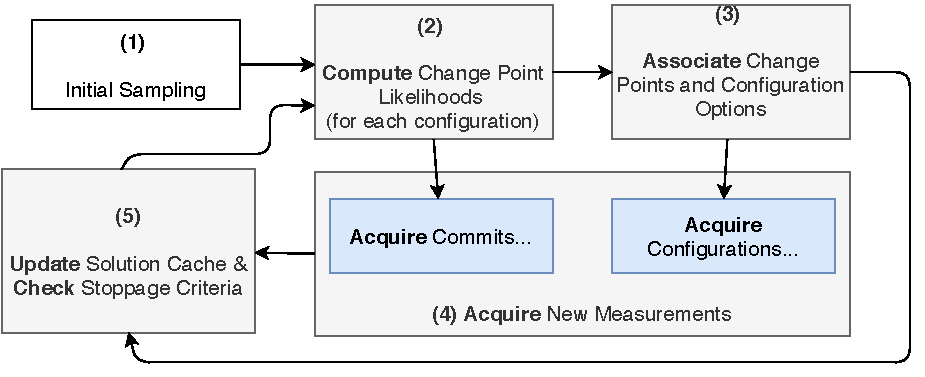
\includegraphics[width=\linewidth]{images/ablauf.pdf}
		\caption{Overview of our approach:  \textcircled{1} Selecting training data across configuration space and version history, \textcircled{2} estimating the change point probability distribution per configuration, \textcircled{3} estimating change points as candidate solutions, \textcircled{4} adaptively augmenting the training set, and \textcircled{5} updating the solution cache and evaluating termination criteria.}
		\label{fig:overview}
	\end{figure}
	
	\subsection{Initialization and Sampling}\label{sec:initialization}
	The first step of our approach is to select a sample set of performance measurements. 
	We select a relatively small, but fixed number of configurations, $n_\text{configurations}$. For each configuration, we select a fixed percentage of commits, $r_\text{commits}$, and assess their respective performance.
	The initial sample set in this setup is kept small and may not represent all relationships between configuration options and performance evolution. 
	The rationale is that, to make our approach more scalable, we explore the combined search space and refine the temporal and  spatial (i.e., configuration-related) resolution where necessary. 
	
	For the initial configuration sampling, we use distance-based  sampling~\cite{kaltenecker_distance-based_2019}, which is a form of random sampling that strives for uniform coverage at low cost. 
	In general, uniform random sampling of configurations is considered to yield the most representative coverage of a configuration space, but it is prohibitively expensive for real-world configurable software systems with constraints among options (i.e., not all combinations of configuration options are valid configurations). 
	Distance-based sampling addresses this problem by demanding the number of selected options to be uniformly distributed to avoid local concentration. 
	
	The key idea of our algorithm to iteratively augment the training set addresses two issues: (1) The configuration space exhibits exponential complexity. 
	(2) Interactions of higher degrees (i.e., interactions involving two or more configuration options) are possible, but relatively rare among configurable software systems~\cite{kolesnikov_relation_2019,kolesnikov_tradeoffs_2019}. Therefore, instead of exhaustive sampling with respect interaction degrees, we iteratively add new configurations to our training sample to search previously undetected influences of options and interactions.
	
	For each configuration in our sample set, the algorithm selects a small number of commits (e.g., one or two percent of all commits) for which it measures performance. 
	The rationale of having only few commits is that, given a relatively large number of configurations, many similar configurations will exhibit change points of the same cause. 
	We mitigate the poor temporal resolution by selecting the commits independently. 
	Compared to a fixed sample of commits across all configurations, this way, each commit is more likely to be measured, at least, once. That is, we obtain change-point estimations for related configurations from independent training samples. 
	For instance, consider the third change point in the introductory DBMS example: 
	At commit 80, all configurations exhibit a performance change. If we sampled two commits, 70 and 90, for all configurations, all that we would learn is that there is a change point somewhere between these two versions. 
	Instead, our approach samples the commits 70 and 90 for the first two configurations, and commits 75 and 95, as well as 65 and 85 for the remaining two configurations respectively. 
	Our best guess then is to assume a change point between commits 75 and 85 since all measurements agree with this conclusion. 
	This way, we increase the temporal resolution while keeping the overall number of performance measurements manageable.
	
	\subsection{Iteration: Change Point Likelihoods}\label{sec:changepointlikelihood}
	For each configuration in our sample set, we estimate the probability of each commit being a change point for the corresponding configuration.
	To this end, we need to define what counts as a performance change. We use a user-defined threshold, which discriminates between measurement noise and performance changes such that different application scenarios as well as system-specific peculiarities can be accounted for.
	If the performance difference for a configuration between two commits exceeds this threshold, we count this difference  as a performance change.
	Although manually defined, there are several possibilities to estimate this threshold automatically.
	Prior to learning, the measurement variation obtained by the repeating measurements for the same configuration multiple times can be estimated and employed as a minimum threshold.
	In addition, a relative or absolute threshold can be derived from the application context, such as a ten percent or ten seconds increase in execution time.
	
	We encode the threshold in a step function $\theta_\tau$:
	\begin{equation}\label{eq:theta}
	\begin{gathered}
	\theta_\tau(a, b) = \begin{cases}
	0,\quad \vert\pi(a) - \pi(b)\vert < \tau\\
	1,\quad \vert\pi(a) - \pi(b)\vert \geq \tau
	\end{cases}\quad a, b \in V, \tau \in \mathbb{R}
	\end{gathered}
	\end{equation}
	The function evaluates to $1$ if the difference between performance $\pi_a$ and $\pi_b$ of commits $a$ and $b$ exceeds the threshold $\tau$ and $0$ if not.
		
	Given a pair of commits, we can now decide whether performance has changed somewhere between the two commits.
	However, not each pair of commits is equally informative.
	The farther the distance between two commits, the lesser the information we can obtain, as there might be several change points in between. 
	In addition, the effect of one change point between two commits can be shadowed by another change point in the opposite direction, such as that one change point increases the execution time and a second decreases the execution time again.
	We define the influence of each pair on our estimation by weighing each pair inversely proportionally to the distance between two commits.
	
	\begin{equation}\label{eq:cpp}
	\begin{gathered}
	p'(v) = \sum_{\lbrace a \in V \vert~ a < v\rbrace} \sum_{\lbrace b \in V \vert~ b > v\rbrace} \underbrace{\theta_\tau(a, b)}_{\text{step function}} \cdot \underbrace{(a-b)^{-2}}_{\text{weighting term}}
	\end{gathered}
	\end{equation}
	
	\begin{equation}\label{eq:normalize}
	\begin{gathered}
	p(v) = \frac{p^\prime(v)}{\sum_{i=1}^{n} p'(i)}
	\end{gathered}
	\end{equation}
	
	For a given commit $v\in V$, we can now estimate a change point probability by comparing each pair of commits before and after $v$.
	This is illustrated in Equation~\ref{eq:cpp}, where $p'(v)$ is the sum of the influence times the performance change indicator $\theta_\tau$ for each pair of commits.
	In practice, however, measuring all commits $V$ is undesirable.
	Therefore, we sample a small number of commits $T \subset V$ instead and compare each pair of commits before and after $v$ to obtain an approximation of $p'(v)$.
	Last, to obtain a proper probability distribution, we need to normalize each value $p'(v)$, as illustrated in Equation~\ref{eq:normalize}.
	Consequently, we obtain an approximation $p(v)$ that represents a probability distribution with $\int_0^{\vert V\vert} p(v)\ d\,v = 1$. The resulting probability distribution as well as its approximation are illustrated in Figure~\ref{fig:cpp_example}, where each change point corresponds to a peak in the probability distribution.
	
	\begin{figure}
		\centering
		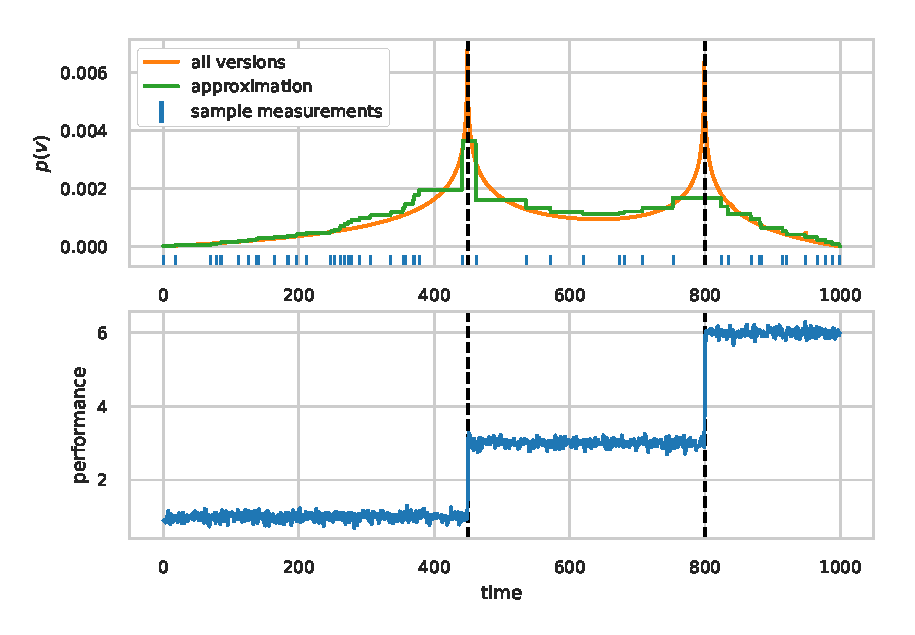
\includegraphics[width=\linewidth]{images/cpp_example.eps}
		\caption{Performance history with 1,\,000 commits and two change points (bottom); Ground truth and approximated change point likelihood $p(v)$ (top)}
		\label{fig:cpp_example}
	\end{figure}
	
	\subsection{Iteration: Assembling a Candidate Solution}\label{sec:candidatesolution}
	We now have change point likelihood estimations for all configurations in our sample set. 
	Different configuration options and interactions contribute to this change point likelihood as we have seen in the introductory DBMS example. 
	In the following step, we estimate the coordinates (pair of commit and configuration option) of likely change points. 
	So, we first estimate candidate commits based on the change point likelihood from the previous step. 
	Then, we associate these candidate commits with configuration options.
	
	\subsubsection{Candidate Commits}
	For each configuration, we compute an approximation of the change point likelihood over commits (cf. Figure~\ref{fig:cpp_example}) to identify local maxima (peaks). We select such peaks under the condition that the peak change point likelihood is greater than a threshold:
	{\color{indigo}\begin{equation}
	\begin{gathered}
	t_\text{CPL} = \frac{1}{\vert V\vert} + N_\text{CPL} \cdot \underbrace{\sqrt{\frac{1}{\vert V\vert} \cdot \sum_{v \in V} \Big(\frac{1}{\vert V\vert} - p'(v)\Big)^2}}_{\text{standard deviation of }p'(v)}
	\label{eq:t_cpl}
	\end{gathered}
	\end{equation}
	% genauere Erklärung, was mit der STDEV gemeint/ausgedrückt wird
	
	The threshold $t_\text{CPL}$ is the average change point likelihood over all commits plus a factor $N_\text{CPL}$ times its corresponding standard deviation over all commits. 
	The factor $N_\text{CPL}$ (default value: 3) allows us to filter peaks that do not stand out enough and might be false positives. The greater $N_\text{CPL}$ is, the stricter the filtering of peaks. That is, for each configuration in our learning set, we obtain a set of commits (configuration-specific candidate commits) that represent possible change points.
	}To reduce variation among the obtained commits, we cluster the commits using kernel density estimation (KDE). The purpose of KDE in our setting is to estimate the probability mass function of whether a commit is a change point. The local maxima of this KDE, subsequently, represent our set of candidate commits. Note that, if two distinct change points are almost coincident commit-wise, they can be mistakenly identified by our approach as one change point that, subsequently, can be associated with configuration options belonging to the two individual change points.
	
	\subsubsection{Associating Commits and Options}
	For each candidate commit that we obtain, we want to know which configuration options are most likely responsible for the respective peak. Hence, we estimate the influence  of each configuration option on the change point likelihood. The core idea is to train a linear model $M: [0,1]^{n_{\text{options}}} \rightarrow [0,1]$, in which each configuration option's coefficient corresponds to its influence. 
	
	Instead of an ordinary linear regression model, we use a linear model that implements the $L_1$ norm for regularization (LASSO). In addition to the least squares penalty, this technique favors solutions with more parameters coefficients set to zero.
	This technique is commonly used to help prevent over-fitting, decrease model complexity, and eliminate non-influential model parameters (configuration options, in our case)~\cite{lasso}. The effect of $L_1$ regularization in a model is specified by an additional hyper-parameter $\lambda$. We tune this hyper-parameter using threefold cross-validation.
	
	For each model (for a candidate commit), we consider a configuration option as associated with a commit, if its influence $c_i$ (i.e., the absolute value of its coefficient) is greater than a threshold:% $t_\text{influence}$:
	{\color{indigo}\begin{equation}
	\begin{gathered}
	t_\text{influence} = \frac{1}{n_\text{options}} + N_\text{influence} \cdot \underbrace{\sqrt{\frac{1}{n_\text{options}} \cdot \sum \Big(\frac{1}{n_\text{options}} - c_i\Big)^2}}_{\text{standard deviation of } c_i}
	\label{eq:t_influence}
	\end{gathered}
	\end{equation}
	The parameter $N_\text{influence}$ (default value: 3) allows us to filter only estimations with low variation. If the intercept of a model exceeds this threshold, we consider this candidate commit a change point that is not configuration-specific (i.e., it affects all configurations). The outcome is a list of \emph{associations}: pairs of candidate commits and (likely) influential configuration options. }
	% unklar, warum N_influence hier eingeführt wird
	
	\subsection{Iteration: Acquiring New Measurements}\label{sec:acquisition}
	The last step in each iteration is the acquisition of new measurements. We extend the existing sample with both new commits for configurations already sampled as well for an additional set of new configurations. The role of including new data is twofold. First, previously assessed configurations or commits might not have captured unseen performance shifts. Therefore, a portion of new data is acquired without further knowledge (exploration). Second, a candidate solution might over- or under-approximate associations and can contribute to the algorithm's overall estimation. Therefore, sampling the second portion of data is guided by exploiting each iteration's candidate solution (exploitation).
	
	\subsubsection{Acquiring Commits}
	The exploration of new commits follows a simple rule: For each configuration, we sample a number commits that exhibit the maximum distance to already sampled commits. 
	
	The exploitation of an iteration's candidate solution employs the estimation of a configuration's change point likelihood (cf. Section~\ref{sec:changepointlikelihood}). We randomly sample among those commits for which the change point likelihood indicates a possible change point, but is not confident. In detail, we select a number of commits for which the change point likelihood is greater than the average (1 divided by the number of commits), but smaller than the average plus the standard deviation of change point likelihood over all commits. By sampling in this range of commits, we incorporate existing knowledge (above average likelihood), but control over-fitting by only sampling commits with maximum likelihood.
	
	\subsubsection{Acquiring Configurations}
	The exploration of new configurations is similar to the initial sample selection strategy (distance-based sampling) described in Section~\ref{sec:initialization}. We select a constant number of configurations (default value: 75) for exploration. 
	
	The exploitation part of acquiring new configurations is guided by the current set of candidate solutions. Each candidate solution describes a change point and associated configuration options. These associated options can be a correct assignment or be an over- or under-approximation. In the latter cases, too many or too few options are associated with a change point. We exploit the existing candidate solutions in a way that addresses both under- as well as over-approximation. We select new configurations using a constraint solver and therefore can specify additional constraints. 
	In the case of under-approximation, too few relevant configuration options are associated with a change point. Given a candidate change point, we require that all associated options keep enabled and that 50\,\% of all not-associated options can be selected. This way, we keep already associated options, but allow new configuration options to be included. Likewise, in the case of over-approximation, too many irrelevant configuration options are associated with a change point. Given a candidate change point, we require that variation only occurs among 50\,\% of the options associated with the change point. That is, we can remove up to 50\,\% of configuration options and narrow down the selection of relevant configuration options.
	
	We limit the total number of new measurements per iteration with a budget $n_\text{measurements}$. This budget is split between acquisition for commits and configurations with a factor $n_\text{commits\_to\_configs} = 0.5$. The measurement budget for commit acquisition is further split between exploration and exploitation with a factor $n_\text{commits\_explore} = 0.5$. That is, initially, 50\,\% of the budget are used for configuration acquisition and 25\,\% for commit exploration and exploitation, respectively. 
	{\color{indigo}As the algorithm proceeds, we multiply the factor $n_\text{commits\_to\_configs}$ by 0.95 and the factor $n_\text{commits\_explore}$ by 0.9. That is, the algorithm shifts  (1) towards sampling configurations in depth and (2) focuses on exploitation in later iterations. The rationale is that we consider pinpointing commit to configuration options a more difficult task than finding performance-changing commits.}
	% zu schnell -> genereller Shift in Richtung exloitation und weg von exploration
	
	\subsection{Solution Cache and Stoppage Criteria}\label{sec:solutioncache}
	After each iteration, we insert the candidate solution in a solution cache. This \textit{solution cache} is a mapping of associations to weights indicating a degree of confidence. 
	The rationale is that, if an association is included repeatedly in an iteration's candidate solution, it is likely a true positive (i.e., a true change point). 
	By contrast, an association that is included only a few times is likely a false positive and can be discarded. 
	We update the solution cache after each iteration in three steps. 
	First, all associations that are either newly included or have been seen before have their weight increased by a constant factor $w_\text{increase} = 1$. Our default value for $k$ is set to 3.
	Second, the weights of all associations in the solution cache are multiplied by a constant decrease factor $e_\text{decrease}\in~\rbrack 0,1 \lbrack$. We set the default value for $e_\text{decrease}$ to 0.3.
	Last, we remove all associations from the solution cache if their weight is smaller than a threshold $t_\text{drop}$. We define $t_\text{drop}$ as the weight an association exhibits if it is included once in a candidate solution but not in $k \in \mathbf{N}$ successive iterations. Effectively, value for $t_\text{drop}$ is $({e_\text{decrease}})^k$ since the increment $w_\text{increase}$ is $1$.
	
	Similarly to the conditions for dropping an association from the solution cache, the algorithm terminates if no association is dropped from the solution cache for $k$ iterations in a row and all association's weights are greater than 1. As a fallback termination criterion, the algorithm also terminates if a user-specified maximum number of measurements $m_\text{max}$ or number of iterations $i_\text{max}$ is reached. 
	
	\section{Evaluation}
	When evaluating our approach with a single experiment, we face a conflict between internal and external validity, a problem that is prevalent in software engineering research~\cite{siegmund_views_2015}. 
	To assure internal validity, the assessment of our approach with respect to accuracy requires prior knowledge of change points as ground truth, which is hardly obtainable as this would require exhaustive performance measurements across commits and configurations. Moreover, to assure  external validity, we require a great degree of variation among subject systems (e.g., number of commits and options, domains of subject systems, etc.) to learn about scalability and sensitivity. 
	So, for a fair assessment, we require not only a large set of systems, but also the respective ground truth performance measurements. The caveat is that it is practically impossible to conduct such exhaustive performance measurements in the large, which was the main reason for proposing our approach in the first place.
	
	To address this dilemma in our evaluation, we conduct two separate experiments, based on synthetic and real-world performance measurements. The first set of experiments uses synthesized performance data providing a controlled experimental setup to assess scalability, accuracy, and efficiency at low cost while simultaneously being able to simulate different scenarios by varying the number of change points and affected configurations in the synthesized data.
	The second sett of experiments uses a batch of real-world performance measurements of three software systems as a necessarily incomplete ground truth to explore whether our algorithm can be practically applied to real-world systems.
	
	With this split experiment setup, we aim at answering the following two research questions:
	\begin{enumerate}[\textbf{$\text{RQ}_{1}$}:]
		\item Can we \emph{accurately} and \emph{efficiently} identify configuration-specific performance change points? 
		\item Can we \emph{practically} identify configuration-specific change points \emph{in a real-world setting}? 
	\end{enumerate}
	
	\subsection{Controlled Experiment Setup}
	We break down the research question $\text{RQ}_1$ into three objectives  to study the influence of the size of configurable software systems, change point properties, and measurement effort.
	
	\subsubsection{Influence of System Size}
	We are interested in how the size of a configurable software system influences the accuracy and efficiency of our approach. 
	To answer this question, we synthesize performance data for systems of varying size in terms of number of configuration options and the number of commits. For the number of configurations $n_\text{options}$, we selected a range that resembles configurable software systems studied in previous work~\cite{muhlbauer_accurate_2019}; likewise, we selected a range for the number of commits $n_\text{commits}$ to cover young as well as mature software systems. We present the ranges of the two size parameters in Table~\ref{tab:synthetic_experiment_ranges}.
	
	\subsubsection{Influence of Change Point Properties}
	A change point may correspond to a single option or an interaction among multiple options. Furthermore, two change points might be only a few or many commits apart. Therefore, for the synthesized software systems, we vary both the total number of change points as well as the degree of interactions that a software system contains. The number of change points ranges from one to ten, reflecting findings of a recent study about performance change points~\cite{muhlbauer_accurate_2019}. We sample the degree of interactions from a geometric distribution (the discrete form of an exponential distribution), which is specified by a single parameter $p$ between 0 and 1, henceforth called $p_\text{interaction}$. The greater the value of $p_\text{interaction}$, the less likely we generate higher-order interactions. The rationale of this setting stems from previous empirical work~\cite{medeiros_comparison_2016,kolesnikov_tradeoffs_2019} that has shown that, by far, most performance issues are related to only single options, or interactions of low degree. We present the specific ranges of the two parameters in Table~\ref{tab:synthetic_experiment_ranges}.
	
	\subsubsection{Influence of Measurement Effort}
	We want to understand how the invested measurement effort affects accuracy and efficiency. An initial sample set chosen too small or large might fail to cover change points to exploit or waste measurement effort. In addition, the number of measurements per iteration can be selected irrespective of the software system size, resulting in too few measurements per configuration, and, thus failing to identify change points. That is, for the initialization of our algorithm, we vary both the initial number of configurations and the number of measurements per iteration. We select the number of configurations in the initial sample set as $n_\text{changepoints}$ times the number of configuration options, and the number of measurements per iteration from a range of three values. We fix the percentage of commits per configuration at 3 percent, which has been a promising sampling rate in previous work~\cite{muhlbauer_accurate_2019}. 
	We present the ranges of the two parameters in Table~\ref{tab:synthetic_experiment_ranges}.
	
	\subsubsection{Operationalization}
	We {\color{indigo}synthesize performance data by initializing each option with a randomly selected influence (cf. coefficients from Equation~\ref{eq:pimodel}) from the range $\left[-1,1 \right]$}. In addition, we randomly select a number of interactions among options to introduce interactions of varying degrees. The interaction degree (i.e., number of selected configuration options) follows a geometric distribution. We assign to each interaction a real-valued influence uniformly from the range $[-1, 1]$. We define six parameter ranges (cf.~Table~\ref{tab:synthetic_experiment_ranges}) for the number of configuration options $n_\text{options}$, the number of commits $n_\text{commits}$, the number of change points $n_\text{changepoints}$, the parameter for the geometric distribution of interaction degrees $p_\text{interaction}$, a factor $N_\text{initial}$, and the number of measurements per iteration $n_\text{measurements}$. The initial number of configurations is the product of $n_\text{options}$ and $N_\text{initial}$. We construct the Cartesian product of all parameter ranges and specify a maximum number of 30 iterations. In addition, we synthesize for each parameter combination in the parameter grid five different software systems by employing different seeds such that no seed is used twice. The total number of experiments with seeds is 10,\,800.% For all synthetic experiments, we specify a maximum number of 30 iterations. 	
	
	\begin{table}
		\centering
		\captionof{table}{Parameter ranges for the synthetic experiment.}
		\label{tab:synthetic_experiment_ranges}
		\begin{tabular}{llr}
			\toprule
			\textbf{}                & \textbf{Parameter}        & \multicolumn{1}{r}{\textbf{Range}} \\
			\midrule
			\parbox[t]{20mm}{\multirow{4}{*}{\rotatebox[origin=c]{0}{\parbox{2cm}{\centering\footnotesize Synthesized Systems}}}} & $n_\text{options}$                & 8, 16, 32, 64                \\
			& $n_\text{commits}$                & 1000, 2500                \\
			& $n_\text{changepoints}$           & 1, 2, 5, 10                        \\
			& $p_\text{interaction}$ & 0.5, 0.7, 0.9                     \\
			\midrule
			\parbox[t]{20mm}{\multirow{2}{*}{\rotatebox[origin=c]{0}{\parbox{2cm}{\centering\footnotesize Initialization}}}}   & $N_\text{initial}$       & 2, 5, 10                           \\
			& $n_\text{measurements}$           & 100, 200, 500                      \\
			\bottomrule            
		\end{tabular}
	\end{table}
	
	For each parameter combination, we record the number of measurements at each iteration, the required number of iterations for termination, as well as each iteration's candidate solution. To assess the accuracy of a parameter combination's outcome (as well as of intermediate iterations), we use the $\text{F}_1$ score, a combination of precision and recall. \emph{Precision} refers to the fraction of correctly identified associations (true positives) among the associations of the retrieved (candidate) solution. \emph{Recall} is the fraction of total number of the relevant associations (i.e., those we intend to find). The $\text{F}_1$ score is the harmonic mean of precision ($P$) and recall ($R$), defined as $\text{F}_1 = 2\cdot\frac{P \cdot R}{P + R}$.	In our context, we defined a correctly identified change point when a commits falls in a narrow 5 commit interval from the ground truth.
	{\color{indigo}To assess efficiency, we employ the required number of iterations for termination and required measurements in relation to the $\text{F}_1$ score as proxy metrics.}
	% schwer zu verstehen
	
	\subsection{Real-World Experiment Setup}
	In the second experiment, we evaluate our approach from a practitioner's perspective, where the properties and whereabouts of change points are unknown.  By means of three real-world configurable software systems, we investigate in particular practical challenges and check whether our algorithm is able to detect performance-relevant commits with respect to configuration options. 
	
	\begin{table}
		\centering
		\captionof{table}{Project characteristics for our three subject systems}
		\label{tab:properties}
		\begin{tabular}{lrr}
			\toprule
			\textbf{Name} & \textbf{\#Options} & \textbf{\#Commits}\\
			\midrule
			\textsc{xz} & 16 & 1193\\
			\textsc{lrzip} & 9 & 743 \\
			\textsc{oggenc} & 12 & 935\\
			\bottomrule
		\end{tabular}
	\end{table}
	
	\subsubsection{Exploratory Pre-Study}
	Of course, we cannot obtain complete ground truth data of our selected subject systems since the search space is exponential in the number of configuration options. 
	However, to provide some context for interpretation of our results, we measured performance for a representative subset of configurations across all commits. To be precise, we sampled configurations using feature-wise, negative feature-wise, pair-wise, and also uniform random sampling strategies, which have been successfully applied to learn performance influences before~\cite{alves_sampling_2020}. We sampled as many random configurations as there are valid configurations sampled with pairwise sampling, which amounts to 79 configurations for \textsc{lrzip}, 152 for \textsc{oggenc}, and 161 for \textsc{xz}. An overview of the three software systems is given in Table~\ref{tab:properties}.
	
	As a workload for the file compression tools \textsc{lrzip} and \textsc{xz}, we used the Silesia corpus, which contains over 200~MB of files of different types. It was designed to compare different file compression algorithms and tools and has been used in previous studies~\cite{muhlbauer_accurate_2019}. For the audio transcoder \textsc{oggenc}, we encoded a raw WAVE audio file of over 60~MB from the Wikimedia Commons collection. For all three subject systems, we assess performance by reporting the execution time.
	
	All measurements were conducted on clusters of Ubuntu machines with Intel~Core
	2 Quad CPUs (2.83~GHz) and 8~GB of RAM (\textsc{xz} and \textsc{lrzip}) and 16~GB of RAM (\textsc{oggenc}). To mitgate measurement bias, we repeated each measurement five times. The coefficient of variation (the ratio of standard deviation and the arithmetic mean) across all machines was well below ten percent. For commits that did not build, we reported the performance measurement of the most recent commit that did not fail to build.
	
	\subsubsection{Operationalization}\label{sec:rq2_operationalization}
	For the actual experiment, we apply our approach on the performance measurements obtained in the pre-study, with a few adjustments.
	First, although our study provides a broad and representative sample set of configurations, we cannot arbitrarily sample valid configurations for a couple of reasons. In particular, these include the commits that do not build as well as hidden configuration options and constraints. While we collected configuration options and constraints thoroughly from documentation artifacts, we cannot assure that our selection is complete. We discuss this limitation further in Section~\ref{sec:discussion}.
	
	Instead, when acquiring new configurations (cf. Section~\ref{sec:acquisition}), we select configurations from our batch of measurements that (1) have not been used already by our algorithm, and (2) are "closest" to the requested configuration (i.e., with the minimal Hamming distance). The rationale is that this allows us to quickly run rapid repetitions with different initializations of our algorithm. Since we employ multiple sampling strategies in our pre-study, we are confident that our broad batch of measurements is representative. Second, we set the number of measurements per iteration $n_\text{measurements}$ to 300. Third, as an initial sample set, we randomly sample 5 configurations from our pre-study set. 
	Last, we initialize our approach with a relative performance threshold $\theta_\tau$ (cf. Equation~\ref{eq:theta}) of ten percent. In the context of the reported relative variation among performance measurements on the machines used, we consider this a rather conservative threshold. 
	We repeat the experiments 10 times with different seeds to quantify the robustness of our approach and to account for the randomness in exploring the configuration space.
	We assess practicality by reporting measurement effort, number of iterations in relation to the pre-study's results, which are based on a vastly greater measurement budget.
	We qualitatively investigate whether the detected commits and options are actually causes of performance changes. That is, we analyze commit messages of the respective repositories for the identified commits to find occurrences of option names or indicators of performance changes. Moreover, we looked into the code changes (e.g., when the commit message just states 'merge') to rationalize about possible performance affecting code changes.
	
	\subsection{Results}	
	\subsubsection{$\text{RQ}_1$ (Controlled Experiment).}
	We illustrate the results of our first set of experiments in Figures~\ref{fig:results_rq1_accuracy_terminated}, \ref{fig:results_rq1_frequency}, and \ref{fig:results_rq1_degree}. The vast majority of experiments terminated within the limit of 30 iterations, as shown in Figure~\ref{fig:results_rq1_frequency}. A small portion of experiments, however, did not meet our termination criteria (more on that below). From all experiments that terminated in Figure~\ref{fig:results_rq1_accuracy_terminated}, we depict the F1 score after they have terminated, that is, after their last iteration\footnote{Due to space limitations we report precision and recall on the paper's companion Web site.}. For most iterations, the mean F1 score falls around or over 0.7, with the first quartile  only slightly being as low as 0.5 (at iteration 29).  In the grand scheme of things, the vast majority of experiments terminated with reasonably high F1 score. 
	\begin{figure}
		\begin{subfigure}{\linewidth}
			\centering
			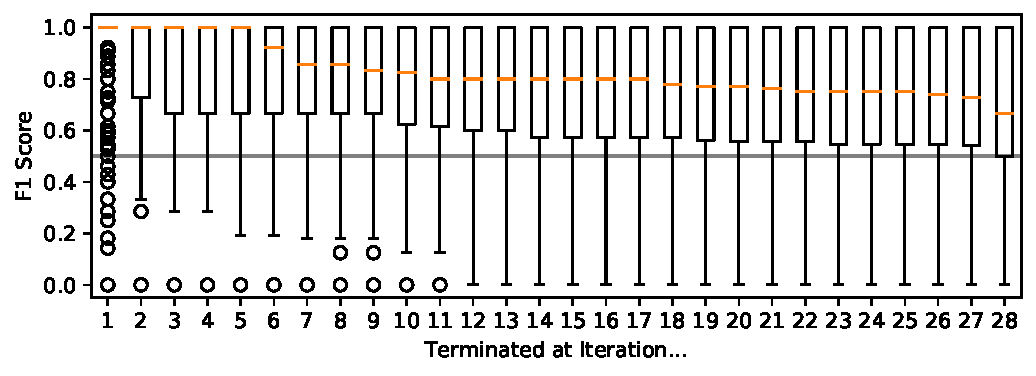
\includegraphics[width=\linewidth]{images/accuracy_after_termination.pdf}
			\vspace{-5mm}
			\caption{F1 score of experiments terminating at different iterations.}	
			\label{fig:results_rq1_accuracy_terminated}
		\end{subfigure}
		\begin{subfigure}{\linewidth}
			\centering
			\vspace{1mm}
			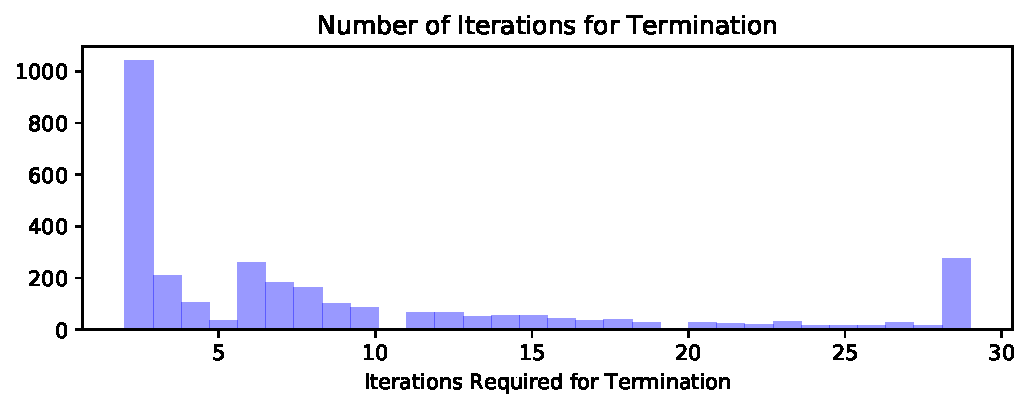
\includegraphics[width=\linewidth]{images/iterations_for_termination.pdf}
			\vspace{-5mm}
			\caption{Frequency of experiments terminating at different iterations.}	
			\label{fig:results_rq1_frequency}
		\end{subfigure}
		\begin{subfigure}{\linewidth}
			\vspace{4mm}
			\centering
			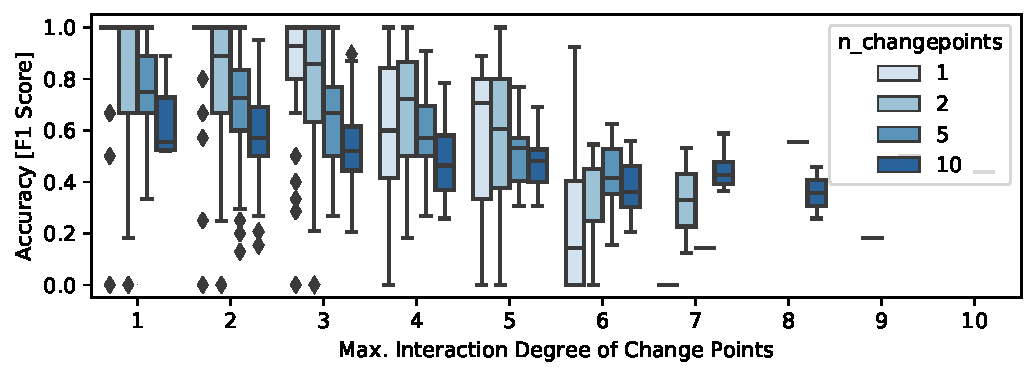
\includegraphics[width=\linewidth]{images/max_degree_after_termination}
			\caption{Influence of the number of change points and interaction degree on accuracy}	
			\label{fig:results_rq1_degree}
		\end{subfigure}
		\caption{Result for the synthetic experiment}
		\label{fig:results_rq1:results_rq1_degree}
	\end{figure} 	
	Regarding measurement effort, for small systems with 8 configuration options, we required up to 50\,\% of all possible measurements. For greater systems, the required measurement effort was well below 1\,\%. The high reported measurement effort for smaller systems is due to our choice of the measurements per iterations, which vastly over-approximates. Since we are able handle systems with more configuration options with similar effort, we are confident that a smaller number of measurements per iteration would reduce the relative measurement effort required substantially.
	
	In Figure~\ref{fig:results_rq1_degree}, we decompose the reported F1 scores to learn how the number of change points or the interaction degree influence our approach. The x-axis shows the highest interaction degree of change points for an experiment run. For interactions of a degree up to 5, the F1 score is mostly above 0.5. We observe a downward trend in the boxplots: the more change points a system contained, the less accurate our algorithm's prediction is.
	
	For the experiments not terminating within limit (the rightmost bar in Figure~\ref{fig:results_rq1_frequency}), we conducted an additional analysis. We compared whether and how the parameter setting of Table~\ref{tab:synthetic_experiment_ranges} explains this non-termination. One setting stands out as the cause for not finishing the experiment within 30 iterations: the number of measurements per iterations. The lower the number of measurements ($n_\text{measurements}$), the more iterations our approach needs.
	\vspace{2mm}
	\greybox{
		\textbf{Summary ($\text{RQ}_1$)}: We are able to identify and pinpoint config\-uration-specific performance change points accurately and at scale. The number of measurements per iteration is the main factor influencing how fast our algorithm terminates.
	}
	
	\subsubsection{$\text{RQ}_2$ (Pre-Study)}
	For our three subject systems, we have manually identified a number of commits, for which performance chang\-ed substantially. We have found 7 change points for \textsc{lrzip}, 2 for \textsc{xz}, and 2 for \textsc{oggenc}. For \textsc{lrzip}, 5 of 7, and for \textsc{xz}, 2 of 2 performance changes affect multiple configurations. By contrast, 2 change points for \textsc{lrzip} affect all measured configurations. All of the measured configurations for \textsc{oggenc} show a shift in performance. That is, the identified change points for \textsc{oggenc} as well as the two for \textsc{lrzip} are likely not configuration-specific. 	
	To further understand possible relations of change points with configuration options, we searched in commit messages for clues. We discuss two notable findings. 
	
	For \textsc{xz}, the commit messages for both change points referenced three particular configuration options (\textsf{hc3}, \textsf{hc4}, \textsf{MatchFinder}). For \textsc{lrzip}, one commit message references configuration option (\textsf{zpac}). Four of seven commit messages contained keywords relating to performance. Two examples are the following:
	
	\begin{quotation}
		"\texttt{\footnotesize liblzma: Adjust default depth calculation for \textbf{HC3} and \textbf{HC4}. [...]}" (revision 626 of \textsc{xz})\\\\
		"\texttt{\footnotesize Use ffsl for a \textbf{faster} lesser\_bitness function.}" (revision 521 of \textsc{lrzip})
	\end{quotation}
	
	Of the remaining 6 commits for \textsc{lrzip}, we identified one as a successor to a merge commit. Within the related pull request\footnote{https://github.com/ole-tange/lrzip/commit/1203a1853e892300f79da19f14aca11152b5b890}, we discovered that the configuration \textsc{lzma} was set to be ignored. This plausibly corresponds to an observed performance shift for configurations with this option enabled. However, this orphan configuration option results in an inconsistent configuration interface, which we discovered with our approach. 
	
	\subsubsection{$\text{RQ}_2$ (Real-World Performance Data)}
	Across the repetitions of our experiments, we found a number of candidate solutions close to the two change points commits for \textsc{xz} and \textsc{oggenc}, respectively, on average after, 3 to 5 iterations. After more than five iterations, the majority of repetitions pinpointed commits correctly within our narrow 5 commit interval. By contrast, for \textsc{lrzip}, we required up to fifteen iterations to reach this temporal precision. Note that, for \textsc{lrzip}, the number of change points is more than three times greater than for the other two software systems. In addition, three pairs of change points are 10 commits or less apart, which led to falsely identified commits. 
	
	The association of commits to configurability, with the exception of \textsc{oggenc}, is inconclusive. For \textsc{oggenc}, our approach consistently reported both change points as not configuration-related. For \textsc{lrzip}, the reported associations included a variety of possible options, but did not converge and report solutions in line with our pre-study. For \textsc{xz}, the majority of association configuration options were „match finder“ options referenced in the commit messages.
	
	We attribute the inconclusive results for \textsc{lrzip} in part to the inconsistency of the configuration interface. For both \textsc{xz} and \textsc{lrzip}, many configuration options are alternatives. That is, for a functionality such as the compression algorithm, only one of the available options can be selected. In our approach, we employ Lasso regression for automated feature selection. This regression model might, given only a small configuration sample, have difficulties with attributing a change point to multiple alternative configuration options and rather opt for one instead.  %Across the repetitions of our experiments, we have found candidate solutions close to the two change points commits for \textsc{xz} and \textsc{oggenc}, respectively, on average, after 3 to 5 iterations. After more than five iterations, the majority of repetitions pinpointed commits correctly within our narrow 5 commit interval.
	\vspace{2mm}
	\greybox{
		\textbf{Summary ($\text{RQ}_2$)}: Our approach is able to precisely link change points to commits with real-world data. Manually associating commits with configuration options worked in many cases, whereas the automated analysis was inconclusive due to incomplete data in the repositories. We observed, at least, one inconsistency in the configuration interface of one subject system.
	}
	
	\section{Discussion}\label{sec:discussion}
	\paragraph{Efficiency} Among all experiments conducted with our synthetic setup, our approach yielded reasonable to high accuracy across most parameter settings. A subsequent analysis of parameter settings showed that our algorithm is not limited by the size of a problem space, but rather the number of measurements per iteration. 
	% mehr Interpretation, Details ausblenden
	{\color{indigo}Our algorithm found multiple change points across settings of up to 2,500 commits and and 2$^{64}$ configurations, resulting in a search space of about $4.6 \cdot 10^{22}$ possible measurements.
	In the context of not more than 5,000 measurements per iteration, the maximum number of measurements (after 30 iterations) added to the initial set of measurements is 150,000. For a setting with 2,500 commits, this represents around $1.4 \cdot 10^{-6}$\,\% and $3.2\cdot 10^{-16}$\,\% of possible measurements for settings with 32 and 64 options, respectively. The vast majority of cases terminated in early iterations.} Hence, we are confident that our approach scales and can efficiently approximate change points for large software systems. Notably, we are able to reproduce this finding in real-world settings when identifying the temporal location of change points. For our controlled experiment setup, we have not tuned the algorithms’ parameters to reach optimal efficiency or accuracy. However, even without tuning, we demonstrated the feasibility and efficiency of our approach. Project-specific fine tuning of several parameters is a possible extension to our approach and can further improve our results.
	
	\paragraph{Pinpointing Configuration Options}
	The synthetic setup has shown that our algorithm can conceptually handle both time and space. We were able to precisely identify commits for which performance changed substantially. By contrast, we were not able to fully reproduce this in a setting with real-world data when attempting to pinpoint change points to configuration options. Possible explanations in the case of \textsc{lrzip} include a partly inconsistent configuration interface. 
	The reason for that is not a limitation of our approach, but missing information in the real-world data (which makes the synthetic setup so important). So, we have documented that, given a precisely identified commit, we can link the affected files to configuration options with little effort. In turn, given a set of code segments of a commit, matching this with the overall code base has been extensively studied before under the umbrella of feature location~\cite{hill_which_2013}.
	Inconsistencies in the documentation of configuration options is a well known and prevalent problem~\cite{rabkin_static_2011}. Our approach might be a means to complement existing feature location techniques with information about configuration-dependent performance changes. 	
	In our latter experiment, instead of directly sampling new arbitrary configurations, we used a finite set of configurations as a proxy (cf.~Section~\ref{sec:rq2_operationalization}). This does not reflect the original layout of our algorithm, but lets us efficiently explore some limitations of this approach. We have learned that, for interpreting the results of our approach, domain knowledge is advantageous as we have identified incomplete and inconsistent configuration interfaces as possible limiting factors. We acknowledge that, while our approach performs well as an automated pipeline in a controlled environment, for real-world applications, a semi-automated setup with additional manual measurement prioritization and deeper knowledge of configuration constraints would improve the applicability of our approach. This is a promising further avenue of future work.
	
	\paragraph{Threats to Validity}
	Threats to \emph{internal validity} include measurement noise that may distort change point approximation. We mitigate this threat by repeating each measurement five times and reporting the mean. With respect to the mean performance, the reported variation was below 10\%. For RQ2, we considered only performance changes of, at least, 10\%. We conducted a pre-study, where we manually identified change points.
	Hence, we are confident that our raw data are robust against outliers. The setup in RQ2 relies on a limited set of previously sampled configurations instead of actively acquiring new ones. We mitigate this limitation by selecting a broad set of configurations in our pre-study with different sampling strategies. We sampled as many randomly selected configurations as there are pairs of configuration options, resulting in a reasonably high coverage of the configuration space. 
	
	Regarding \emph{external validity}, we cannot claim that we have identified all limitations possibly arising in a practical setting. However, we selected popular software systems that are well optimized for performance and often make use of configuration options to tune performance.  Although we have shown possible limitations in a practical setting, our results, in conjunction with our exhaustive synthetic study, are reproducible, and we were able to test corner cases and assess scalability so that we believe that our results hold for many practical use cases.
	
	\section{Related Work}\label{sec:rw}
	\paragraph{Performance-relevant Commits} Identifying performance-changing commits is a prevalent challenge in regression testing, often applying change point detection algorithms on batches of performance observations~\cite{cityIdentifying2014,daly_industry_2020}. A way to reduce testing overhead is to employ only a fraction of performance observations or to prioritize commits. Alcocer et al. assess performance for uniformly selected commits to estimate the risk of a performance change introduced by unobserved commits~\cite{sandoval_alcocer_learning_2016,alcocer_prioritizing_2020}. Huang et al. estimate the risk of performance changes solely based on static analysis of individual commits to prioritize commits for regression testing without assessing performance~\cite{huang_performance_2014}. Mühlbauer et al. use Gaussian Processes and iterative sampling to learn performance histories with few performance observations~\cite{muhlbauer_accurate_2019}. They extract performance changing commits by applying change point detection algorithms to learned performance histories. All of the above approaches reduce testing overhead, but do not address the performance across different configurations of software systems. Our approach incorporates performance changes across different configurations by leveraging similarities in related configuration's performance histories.
	
	\paragraph{Performance of Configurable Software Systems} Associating configuration options and interactions with their influence on performance is a conceptual basis for our work. There exists extensive work on modeling configuration options as features for machine learning, such as classification and regression trees~\cite{guo_2018_data,guoVariabilityawarePerformancePrediction2013,sarkarCostEfficientSamplingPerformance,nairUsingBadLearners2017}, multi-variable regression~\cite{siegmundPerformanceinfluenceModelsHighly2015}, and deep neural networks~\cite{haDeepPerf2019}. Predictive models for software performance can be used to find optimal software configurations~\cite{nairFlash18}.
	In contrast to learning performance for arbitrary configurations, our approach aims at finding  performance changes, and subsequently, pinpointing them to configuration options and interactions.
	A similar scenario to ours has been studied by Jamshidi et al.~\cite{jamishidi_transfer_2017,jamshidi_transfer_gp_2017,jamshidi_learning_2018}. Between software versions, the performance influence of only few configuration options changes. The authors propose two approaches for learning a transfer function between performance models of different environments, such as versions, based on Gaussian Processes~\cite{jamshidi_transfer_gp_2017} and progressive shrinking the configuration space~\cite{jamshidi_learning_2018}. We see great potential for future work in applying Gaussian Processes to our problem.
	
	\section{Conclusion}
	% sperrig laut sven
	{\color{indigo}Changes in the observed performance of a software system can be configuration-specific and difficult to pinpoint to configuration options and commits. We combine both two orthogonal perspectives, the commit history and configurability of software systems to pinpoint performance changes to individual commits and configuration options. 
	We propose an iterative sampling approach that leverages similarities in performance histories of related configurations to identify performance shifts precisely and, subsequently, pinpoint them to configuration options and interactions. 
	We have shown with a synthetic data set that our approach is sound and able to identify performance change points accurately and at scale. Experiments with three configurable software systems confirm the temporal precision of our approach and have confirmed prevalent practical challenges when studying real world-software systems. It is an avenue for further research to incorporate further information, such as commit artifacts, when pinpointing performance changes.}
	
	\section{Acknoledgements}
	Apel’s work has been supported by the Deutsche Forschungsgemeinschaft (DFG) under the contract AP 206/11-1. Siegmund’s work has been supported by the DFG under the
	contracts SI 2171/2 and SI 2171/3-1.
	
	\clearpage
	
	%\clearpage
	%%
	%% The next two lines define the bibliography style to be used, and
	%% the bibliography file.
	\bibliographystyle{ACM-Reference-Format}
	\bibliography{extracted}
	\clearpage
	
	
\end{document}
\endinput
%%
%% End of file `sample-sigconf.tex'.
